%!TEX root = ../dissertation.tex

\chapter{Some extra stuffs}

Here is some extra stuff.


\section{Standalone Package}

When draw some figure with \texttt{Tikz}, it is nicer to try out the drawing
in the small "test bench" rather than do the drawing in the main dissertation
latex project and compile the whole document again and again.

The \texttt{standalone} package provides the possibility of putting the figure
environments to their own source code files and compiling them in a small "test
bench" main file: \texttt{standalone\_test.tex}.

The figure environments can be put to the dissertation document using
\inlinecode{Tex}{\\input\{\}} command.
As an example, \autoref{fig:standalone} is included here with:

\begin{spacing}{1}
\begin{lstlisting}[language={[LaTex]Tex}]
\begin{figure}[!h]
	\centering
	\documentclass[tikz, varwidth=true]{standalone}
\begin{document}
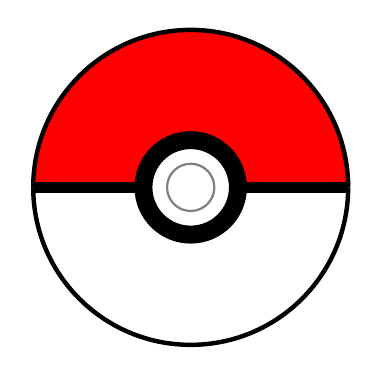
\begin{tikzpicture}[font=\small\sffamily, >=latex, thick]

	%% draw help lines
	% \draw[step=0.5, help lines] (-2.4,-2.4) grid (2.4,2.4);

	\filldraw [ultra thick, fill = red] (2.0,0) arc [start angle = 0, end angle = 180, radius = 2.0] ;
	\filldraw [ultra thick, fill = white] (-2.0,0) arc [start angle = 180, end angle = 360, radius = 2.0] ;

	\draw[line width=4.0] (-2.0,0) -- (2.0,0);

	\filldraw[fill=black] (0,0) circle [radius = 0.7];
	\filldraw[fill=white] (0,0) circle [radius = 0.5];
	\draw[gray] (0,0) circle [radius = 0.3];

\end{tikzpicture}
\end{document}

	\caption{A drawing of pokemon ball.}
	\label{fig:standalone}
\end{figure}
\end{lstlisting}
\end{spacing}

\begin{figure}[!h]
	\centering
	\documentclass[tikz, varwidth=true]{standalone}
\begin{document}
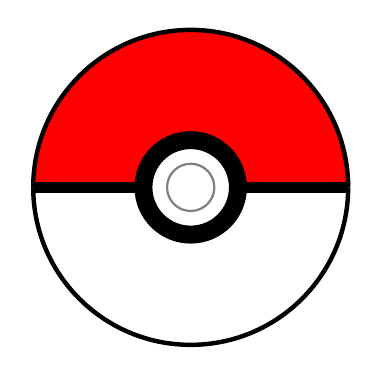
\begin{tikzpicture}[font=\small\sffamily, >=latex, thick]

	%% draw help lines
	% \draw[step=0.5, help lines] (-2.4,-2.4) grid (2.4,2.4);

	\filldraw [ultra thick, fill = red] (2.0,0) arc [start angle = 0, end angle = 180, radius = 2.0] ;
	\filldraw [ultra thick, fill = white] (-2.0,0) arc [start angle = 180, end angle = 360, radius = 2.0] ;

	\draw[line width=4.0] (-2.0,0) -- (2.0,0);

	\filldraw[fill=black] (0,0) circle [radius = 0.7];
	\filldraw[fill=white] (0,0) circle [radius = 0.5];
	\draw[gray] (0,0) circle [radius = 0.3];

\end{tikzpicture}
\end{document}

	\caption{A drawing of pokemon ball.}
	\label{fig:standalone}
\end{figure}

\section{Adding Annotation to figure}

A snippet of adding annotations to the figures can be found in
\emph{appendix/annotation.tex}.
The help lines and the coordination is drawn for adding annotations.
The help lines and the coordination can be turned off after adding the
annotations.

With the help lines and coordination, the figure shown in
\autoref{fig:annotation}.
\begin{figure}[!h]
	\centering
	%%%% snippet to add annotation to a figure
%%%% reference: https://tex.stackexchange.com/questions/9559/drawing-on-an-image-with-tikz
\documentclass[tikz, varwidth=true]{standalone}
\begin{document}
\begin{tikzpicture}[font = \normalsize \sffamily, align = center]
	\node[anchor = south west, inner sep = 0] (image) at (0,0) {
		
\includegraphics[width=0.45\textwidth]{appendix/figures/pokemon_ball.pdf}};
	\begin{scope}[x = {(image.south east)}, y={(image.north west)}]

		%% draw help lines
		\draw[help lines,xstep=.1,ystep=.1] (0,0) grid (1,1);
		\foreach \x in {0,1,...,9} { \node [anchor=north] at (\x/10,0) {0.\x}; };
		\foreach \y in {0,1,...,9} { \node [anchor=east] at (0,\y/10) {0.\y}; };

		%% add nodes
		\node[anchor = south] (up) at (0.8, 1.05) {Upper half sphere};
		\node[anchor = south] (down) at (0.2, 1.05) {Lower half sphere};
		\node[anchor = south] (trigger) at (0.5, 1.05) {Trigger};

		%% draw arrows
		\draw[->, thick] (up) -- (0.7, 0.8);
		\draw[->, thick] (down) -- (0.3,0.3);
		\draw[->, thick] (trigger) -- (0.5,0.5);

	\end{scope}
\end{tikzpicture}
\end{document}

	\caption{Example of Adding Annotation to Figure.}
	\label{fig:annotation}
\end{figure}


\section{Big O}

The "Big O", the order of, is show as $\mathcal{O}$ using the math font provided by
\emph{newtxmath} package.
In order to get the symbol like $\bigO$, a new symbol is declared using the
Computer Modern math font in \emph{setup/macros.tex}:
\begin{spacing}{1}
\begin{lstlisting}[language={[LaTex]Tex}]
\DeclareSymbolFont{cmfonts}{OMS}{cmsy}{m}{n}
\DeclareMathSymbol{\cmbigO}{\mathord}{cmfonts}{`O}
\newcommand{\bigO}{\mathcal{\cmbigO}}
\end{lstlisting}
\end{spacing}

\inlinecode{Tex}{\$\\mathcal\{O\}\$} produces $\mathcal{O}$, and
\inlinecode{Tex}{\$\\bigO\$} produces $\bigO$.
